%
% 25-Fpq.tex
%
% (c) 2023 Prof Dr Andreas Müller
%

%
% Der Faktor F(p,q,\omega)
%
\subsection{Der Faktor $F(q,p,\omega)$}
Der zweite Faktor der Faktorisierung von $\mathscr{F}_{pq}$ ist die Matrix
\begin{equation}
\def\h{2}
\def\punkt#1#2{({(#2)*\h},{-(#1)*\h})}
\def\einheit#1#2{
	\fill[color=gray!40] \punkt{#1-0.5}{#2-0.5}
	-- ++({0.05*\h},0) -- ++({0.95*\h},{-0.95*\h})
	-- \punkt{#1+0.5}{#2+0.5}
	-- ++({-0.05*\h},0) -- ++({-0.95*\h},{0.95*\h}) -- cycle;
}
\def\feld#1#2#3{
	\node at \punkt{#1}{#2}
		{$#3{\color{white}\mathstrut\cdot I_p}\mathstrut$};
}
F(q,p,\omega^p)
=
\left(\raisebox{-5cm}{%
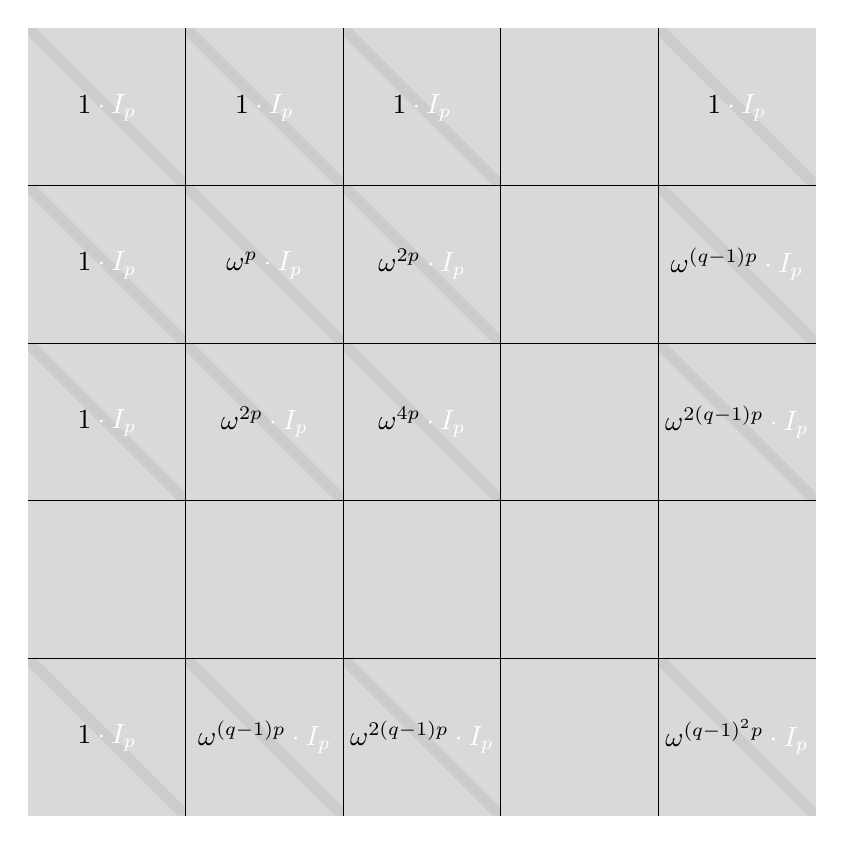
\begin{tikzpicture}[>=latex]
\fill[color=gray!30] \punkt{0}{0} rectangle \punkt{5}{5};
\foreach \x in {0.5,1.5,2.5,4.5}{
	\foreach \y in {0.5,1.5,2.5,4.5}{
		\einheit{\x}{\y}
	}
}
\foreach \x in {1,2,3,4}{
	\draw \punkt{\x}{0} -- \punkt{\x}{5};
	\draw \punkt{0}{\x} -- \punkt{5}{\x};
}
\feld{0.5}{0.5}{1}
\foreach \x in {1.5,2.5,4.5}{
	\feld{\x}{0.5}{1}
	\feld{0.5}{\x}{1}
}
\feld{1.5}{1.5}{\omega^p}
\feld{1.5}{2.5}{\omega^{2p}}
\feld{1.5}{4.5}{\omega^{(q-1)p}}

\feld{2.5}{1.5}{\omega^{2p}}
\feld{2.5}{2.5}{\omega^{4p}}
\feld{2.5}{4.5}{\omega^{2(q-1)p}}

\feld{4.5}{1.5}{\omega^{(q-1)p}}
\feld{4.5}{2.5}{\omega^{2(q-1)p}}
\feld{4.5}{4.5}{\omega^{(q-1)^2p}}
\end{tikzpicture}}
\right).
\label{buch:diskret:vandermonde:eqn:}
\end{equation}
Die Matrix sieht aus wie eine $q\times q$-Fourier-Matrix, allerdings mit dem
Unterschied, dass $p\times p$-Einheitsmatrizen anstelle der einzelnen
Einträge stehen.
Statt der Potenzen von $\omega$ findet man die Potenzen von $\omega^p$.
Da aber $(\omega^p)^q = \omega^n=1$, ist das genau die erwartete Basis
in der Fourier-Matrix $\mathscr{F}_q$.

Mit der Notation des Kronecker-Produktes von Matrizen aus
Abschnitt~\ref{buch:diskret:section:tensor} ist der zweite Faktor
\[
F(q,p,\omega)
=
\mathscr{F}_q
\otimes
I_p.
\]

\begin{satz}
Die Determinante von $F(p,q,\omega)$
ist
\[
\det F(p,q,\omega)
=
\det(
\mathscr{F}_q
\otimes
I_p
)
=
(\det \mathscr{F}_q)^p.
\]
\end{satz}

\begin{proof}[Beweis]
Die Aussage über den Wert der Determinanten folgt unmittelbar aus
dem Satz~\ref{buch:diskret:tensor:satz:deteinheit}.
\end{proof}

